



\section{Harmful Algal Blooms}


%First paragraph. INTRODUCTION GENERIC PARAGRAPH

Harmful algal blooms (HABs) are becoming an increasing issue for drinking and recreational water use.
HABs are a result of over-productivity of phytoplankton biomass which causes the epipelagic zone appear bright green and have negative effects on other organisms \cite{moore_richard_cyanobacterial_1993}. In most cases, HABs are found in coastal regions, streams, and freshwater lakes \cite{rastogi_cyanotoxin-microcystins:_2014}
HABs are diverse, composing an array of  microorganisms ranging from  different species of cyanobacteria, diatoms, algae, and dinoflagellates found worldwide \cite{dittmann_cyanobacterial_2012}.
As an autotroph, HABs can rapidly grow under warm and nutrient-rich conditions \cite{rastogi_cyanotoxin-microcystins:_2014}. Their ability to manipulate buoyancy by modulating the intracellular gas vesicles gives them a competitive advantage over other species for light \cite{feng_how_2018}. HABs can endanger riparian owners of lake estates, recreational swimmers and aquatic organisms. Swimming or contact in any waterbody with HABs can pose a health risk as some HABs can be toxin producing species. In a nationwide survey done by the EPA, 92\% of the state in the US had detectable toxins from HABs (known as cyanotoxins) \cite{noauthor_national_2009}.


% got to say what HABs are in michigan...
%
The ecological harm caused by HABs does not necessarily come from the toxins. Even with no detectable toxins present, there are still implications from HABs. The large biomass of algae can quickly die off due to limiting resources \cite{charlton_oxygen_1980}. Consequently, the abounding biomass is consumed by other microorganisms which, in the process of respiration, depletes dissolved oxygen which renders the aquatic habitat unsuitable.  \cite{anderson_harmful_2002}.




%TOXICITY Cyanotoxins are a dangerous attribute of HABs.





Cyanobacterial toxins are vastly diverse as 600 recognized peptides have been discovered \cite{welker_cyanobacterial_2006}. The variety of toxins have a range of different mechanism of toxicity. One of the most dangerous called saxitoxin are sodium channel blockers, a potent neurotoxin which paralyze and dead from respiratory failure \cite{moore_richard_cyanobacterial_1993}.
Anatoxin-a is also a very dangerous with its potent toxicity. It is known as Very Fast Death Factor(VFDF) due to its ability to irreversibly bind to nicotinic acetylcholine receptors which consequently leading to respiratory failure in a very quickly manner \cite{codd_cyanobacterial_1999, moore_richard_cyanobacterial_1993}.

Microcystin, much of what our survey is focused on, is a small cyclic peptide having a large range of diverse structure. There are over 100 known variation of microcystin with 6 congeners recognized by the EPA are MC-LR, MC-RR and MC-LA \cite{puddick_modulation_2016}. The most frequently occurring congener variant of microcystin is MC-LR \cite{rastogi_cyanotoxin-microcystins:_2014}. Figure \ref{structure1} shows the structure of MC-LR which contains L-luecine (L) and L-Arginine (R). Other amino acids such as alanine (A), tryptophan (W), tyrosine (Y), and phenylalanine (F) can be substituted for other variant congeners. Microcystin have various forms due to different L$-$ammino acids. The main components of microcystin is mostly comprised of D-erythro$\beta$-methylaspatric acid (D-MeAsp), 3-amino-9-methoxy-10-phenyl-2,6,8-trimethyl-deca-4,6-dienoic acid (Adda), \textit{N}-methyldehydro-alanine (Mdha) and other possible variable amino acids \cite{trogen_conformational_1996,nishizawa_genetic_1999}.
Microcystins are produced by a mix of to systems, polyketide synthase(PKS) and nonribosomal peptide synthetase (NRPS) \cite{tillett_structural_2000}.
The genetic mechanism of microcystin synthesis involves multiple protein modules which are responsible for incorporating different amino acids, ultimately creating the cyclic peptide \cite{nishizawa_genetic_1999}.

Cyanotoxins are mostly intracellular, except for the case of cylindrospermonspin, a potent cytotoxin \cite{rastogi_cyanotoxin-microcystins:_2014}. The formation of blooms is usually followed by increase of cyanotoxin due to cell lysis either from cell apoptosis or from mechanical abruption \cite{rohrlack_fate_2007} Many of the species that are producing hepatoxins and neurotoxins in high amounts are killing livestock and wildlife \cite{anderson_harmful_2002}. The possible route of exposure  for humans can be from dermal contact, accidental ingestion, breathing in lake spray aerosols and failure of decontamination in drinking water plants \cite{may_aerosol_2018,codd_cyanobacterial_1999}. Exposure through dermal contact can be an irritant. HABs can create lipopolysaccharide, an endotoxic, which create rashes on upon contact with skin as it triggers a inflammatory response \cite{ moore_richard_cyanobacterial_1993}. Although a rare case, accidental ingestion of microcystin by directly drinking water from an affected lake could  lead to liver failure and eventually causing death \cite{monks_potent_2007}.

State government and health officials continuously monitor and analyze surface and drinking water for microcystin. The World Health Organization (WHO) have guidance level of 1 $\mu$g/mL for drinking water \cite{world_health_organization_guidelines_2003} For the state of Michigan, the USEPA have a draft guidance level for recreational surface water are 4 $\mu$g/mL \cite{us_epa_draft_2016}. Methods of quantifying microcystin will often measure MC-LR Levels above those guidelines requires state officials to issue health advisory not to swim in the effected area.  There are many methods of analysis for detection of either cyanobacteria or the toxins. The common routine methods employed by state agencies are ELISA kits by Abraxxis. This is an antibody method that measures the ADDA-moiety of the microcystin.
The test kit has good cross-reactivity with other congeners.
The test kit uses MC-LR for its calibration standards so the reported value is in terms of MC-LR equivalence.

Lake Erie faced an  issue with a large bloom where massive amounts of fish died off due to the void of oxygen which vastly affected the condition of the lake \cite{charlton_oxygen_1980}. HABs affected over 400,000 people hindering drinking water supply in Toledo, Ohio preventing the citizens to drink or bath from their homes \cite{mann_toledo_2014}. In this case, Maumee river has and its watershed is predominantly agriculture \cite{}. Some studies have mostly shown nutrient enrich conditions usually from agricultural runoff or disturbance of ecological conditions that affect nutrient cycling along with the warm weather causing the massive bloom \cite{ahn_evaluation_2011, ahn_rainfall_2002, anderson_harmful_2002, jiang_statistical_2008}.



Predictive models are useful utility to forecast HABs along coastal environment. Successful forecasting methods employ multiple real-time data along with effective forecast models.  NOAA uses data to predict HABs on the Gulf of Mexico, Lake Erie, and other coastal environments based on satellite data and weather models \cite{kavanaugh_assessment_2013} . Issuing warnings to the public can prevent exposure and be greatly beneficial. They have provide effective forecast, continuously available for the public on their website (\url{https://tidesandcurrents.noaa.gov/hab_info.html}). However, the forecast power is greatly diminished with sattelite imagery when there are cloudy conditions. Forecasting for inland lakes does not work with satellite imagery as the extent of the lake's area will often limit the predictability.



Predictive models based on studied features that contributes to HABs are explored instead, using measured water quality parameters, climate information, and ecological indicators.
Understanding the energy source for cyanobacteria can help to predict HAB occurrences.
Eutrophication is one of the most studied issue in terms of causing HABs. Nitrogen and phosphorus from agricultural runoff is
Nutrients in the form of organic and inorganic forms play a role in biomass production. In controlled experiments, nutrients such as inorganic nitrogen or phosphorus are limiting growth factors when microcystin aereginosa grown in the laboratory \cite{}
Phosphorus is commonly used in bacteria for making their cell walls. Co-polymers with majority of their bonds consisting of phosphodiaster bonds. There are many possible sources of nutrients that can contribute the growth of cyanobacteria and algae. The frequency of HABs around the world have increased, most likely due to the rise of anthropogenic effects such as farming, waste management, and non-point source pollution. \cite{wilhelm_relationships_2011, paerl_controlling_2011}.
The intensity, extent, and spatial coverage has been increasing globally due to more ecological disturbances \cite{codd_cyanobacterial_1999}.  HABs is believed to be largely linked by mostly by agricultural runoff as the source of stimuli \cite{smith_eutrophication_2009}.
Sources from sewage from septic tanks, animal waste and agricultural runoff  could contribute to HABs. Nutrients from agriculture runnoff can have a great effect as fertilizer application has been increasing \cite{anderson_harmful_2002}.

There are many statistical analysis on existing public data. The EPA conducted a large lake survey called the National Lake Assessment  with data collected over 1,000 lakes nationwide.


\begin{figure}[t]
  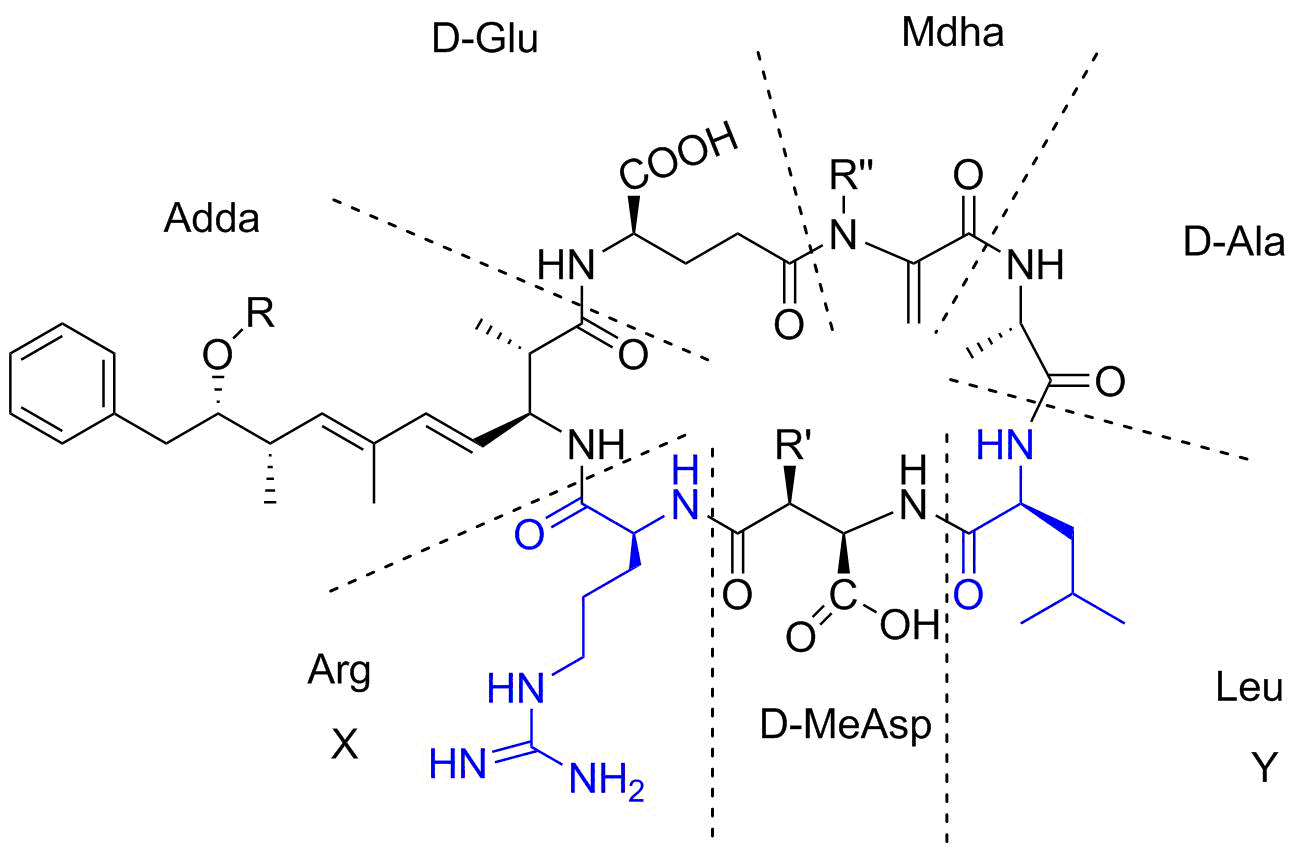
\includegraphics[width=\textwidth]{Microcystin-LR.eps}
  \caption{Structure of MC-LR}
  \begin{flushleft}
  a) Adda group responsible for the hepatoxicity
  b) L-leucine, a variable amino group amongst other congeners
  c) L-arginene, also a variable amino group in other congeners
  d) Methyl-group which can be demethylated in other congeners.
    \end{flushleft}
  \label{structure1}
\end{figure}





\section{Goals and Aims}

In our survey on 29 inland lakes in Michigan, we seek to build a predictive model on microcystins. In addition, we  measured for cylindrospermopsin and anatoxin-a to see if they are present in Michigan. Before the survey, I hypothesized if the lake's watershed is more urbanized areas I would expect higher microcystin concentrations. Developed land can increase nutrient rich runoff which can positive influence algal blooms. Previous studies shown developed areas having a major influence on the occurence of CHABs because of more possible sources like applied fertilizer or leaky septic tanks \cite{beaver_land_2014, anderson_harmful_2002}. Lakes with higher developed areas may also have a possible influence nutrient mobility, which in turn drive microcystin production.

One of our objective is to have a model that is simple and is robust in predicting HABs.
My goal is to explore what drives HABs and build a predictive model based from our collected data.  With the collected observations, I investigated the best possible predictive model from our dataset. Microcystin concentrations from LC-MS/MS and \emph{16S rRNA} gene copies will be tested as the response variable.
Some studies will assess cyanobacterial cell count or mass, concentrations of chloraphyll-a microcystin concentrations as a response variable as its most likely associated with HABs \cite{moore_richard_cyanobacterial_1993, ahn_evaluation_2011, jiang_statistical_2008, beaulieu_nutrients_2013, taranu_predicting_2017}. Cyanobacteria cell counts would be ideal for us to measure whether the lake is exhibiting a bloom. We currently are working on counting cells and unfortunately not completed thus far.  I used microcystin concentration as the main predictor variable of interest. I also observed the \emph{16s rRNA} gene copies as response variables as well as this measures relatively how much cyanobacteria there are based on the amount of 16S rRNA.

My research hypothesis:

\begin{enumerate}
\item Harmful algal blooms is influenced with land use attributes, specifically developed/urban land, which can be used to predict microcystin concentrations
\item Nutrient concentrations can be explained by land use characteristics
\item Identify important features from the collected dataset to build a predictve model for HABs.
\end{enumerate}
